\documentclass[a4paper,11pt]{article}

\usepackage[a4paper,margin=1in]{geometry}
\usepackage[utf8]{inputenc}
\usepackage{amsmath}
\usepackage{amssymb}
\usepackage{amsthm}
\usepackage{booktabs}
\usepackage[small]{caption}
\usepackage{cite}
\usepackage{colortbl}
\usepackage{enumitem}
\usepackage{framed}
\usepackage{graphicx}
\usepackage{multirow}
\usepackage{microtype}
\usepackage[dvipsnames]{xcolor}
\usepackage[unicode]{hyperref}
\usepackage{amsfonts}
\usepackage{algorithm}
\usepackage{algpseudocode}
\usepackage{bm}
\usepackage{mathtools}
\usepackage{subcaption}

\usepackage{listings}
\usepackage{rustlistings}

\bibliographystyle{plainurl}

\setlength{\OuterFrameSep}{0.3ex}
\setlength{\FrameSep}{1.5ex}

\newcommand{\myaff}[1]{\,$\cdot$\, {\small #1}\par\smallskip}
\newcommand{\fakeparagraph}[2]{\par\noindent\textbf{#1}\hspace{1em}#2}

\usepackage{thm-restate}

% Problem definition environment
\newfloat{problemdef}{htbp}{loa}
\floatname{problemdef}{Problem}
\newcommand{\problemcaptionkludge}{\rule[-.3\baselineskip]{0pt}{\baselineskip}}

\theoremstyle{plain}
\newtheorem{theorem}{Theorem}[section]
\newtheorem{lemma}[theorem]{Lemma}
\newtheorem{corollary}[theorem]{Corollary}
\newtheorem{observation}[theorem]{Observation}
\theoremstyle{definition}
\newtheorem{definition}[theorem]{Definition}
\newtheorem{example}[theorem]{Example}
\theoremstyle{remark}
\newtheorem*{remark}{Remark}
\newtheorem{openquestion}[theorem]{Open question}

\newcommand{\tcode}[1]{\rstinline{#1}}
\newcommand{\tperm}[1]{\texttt{#1}}

% Well-parenthesized commands
\newcommand{\set}[1]{\ensuremath{\left\{#1\right\}}}

\newenvironment{myabstract}
{\list{}{\listparindent 1.5em%
        \itemindent    \listparindent
        \leftmargin    0cm
        \rightmargin   0cm
        \parsep        0pt}%
    \item\relax}
{\endlist}

\newenvironment{mycover}
{\list{}{\listparindent 0pt
        \itemindent    \listparindent
        \leftmargin    0cm
        \rightmargin   0cm
        \parsep        0pt}%
    \raggedright
    \item\relax}
{\endlist}

\begin{document}

\begin{mycover}
{\huge\bfseries\boldmath Tree Borrows\par}
\bigskip
\bigskip
\bigskip


Author: \textbf{Neven Villani}
\myaff{ENS Paris-Saclay}

~\newline

Advisor: \textbf{Derek Dreyer}
\myaff{MPI for Software Systems}


Advisor: \textbf{Ralf Jung}
\myaff{ETH Zürich}


\end{mycover}
\medskip

\begin{myabstract}
\fakeparagraph{Abstract.}
\end{myabstract}
\medskip


\section{Introduction}

While the purpose of type systems and typing information in programs is usually
presented as primarily a matter of security (strict type systems can rule out
at compilation-time a number of bugs), they also enable compilers to generate
more efficient code in both space and time. Languages with strict compile-time
type systems can avoid the need for typing metadata at runtime, can have static
dispatch of generic functions, have fewer bounds checks for memory accesses,
or even in the case of Rust eliminate the need for a runtime garbage collector entirely.

In Rust the type system includes aliasing information (mutability and uniqueness),
which is to be used not only for safety guarantees, but also to improve
performance and enable optimizations that are only valid under certain aliasing
guarantees. For example a guarantee of immutability of the data behind a pointer
enables optimizations that would not be valid if the value changed from one read
to the next.
Unfortunately, \tcode{unsafe} code can break these assumptions by allowing at
compile-time accesses through raw pointers that do not respect uniqueness.
This makes a number of desirable optimizations invalid, and it is also an
indicator of subtle bugs.

We aim to define an aliasing model for Rust, which is a runtime semantics
that restores some of the assumptions made impossible in the presence of \tcode{unsafe}
by declaring a certain number of patterns as Undefined Behavior (UB), namely
patterns that violate desirable assumptions. The compiler can then assume
that no UB occurs, which rules out all programs that violate the required
assumptions and enables back the associated optimizations.

\subsection{Motivating example}

As a first concrete example, consider the following function:
\begin{lstlisting}[language=rust]
fn example1(x: &mut u64, y: &mut u64) -> u64 {
     let xval = *x; // First read of *x
     *y = xval + 1;
     let xval = *x; // Second (redundant ?) read of *x
     return xval;
}
\end{lstlisting}

Because mutable references in safe Rust are unique, \tcode{x} and
\tcode{y} must point to disjoint regions of memory. In particular the
instruction \tcode{*y = xval + 1} constitutes a write to \tcode{y}, but it
cannot affect the memory covered by \tcode{x}: the value \tcode{*x} is unaffected
and thus the second read of \tcode{*x} is redundant. This function can be
optimized to perform fewer operations (two fewer loads) by deleting the second line on which
\tcode{*x} is read, without modifying behavior.

However there exists in Rust the \tcode{unsafe} keyword which
allows the programmer to bypass certain compiler checks by extending the
available instruction set: among other things the \tcode{unsafe} keyword allows
dereferencing raw pointers in the following manner:
\begin{lstlisting}[language=rust]
fn context1() {
    let mut data = 42u64;
    let data_ptr = &mut data as *mut u64; // One raw pointer,
    let x: &mut u64 = unsafe { &mut *data_ptr }; // converted into two mutable
    let y: &mut u64 = unsafe { &mut *data_ptr }; // references to the same memory.
    let result = example1(x, y); // Invocation with non-disjoint x and y!
    assert!(result == 43);
}
\end{lstlisting}
Here we use \tcode{unsafe} instructions to obtain two mutable references
to the same location, and we pass both of them to \tcode{example1}.
While in this context the original version of \tcode{example1} will return
\tcode{43}, the optimized version where the second read of \tcode{*x} is removed
will instead return \tcode{42}.
The optimization shown here is thus not unconditionally valid: violating the
uniqueness requirement of mutable references has enabled us to create a program
in which the optimization does not preserve behavior.

However we want this optimization to be valid, on the grounds of \tcode{context1}
being a ``bad'' program that violates the assumption of uniqueness that we want to be able
to make. This issue is solved by adjusting the operational semantics of Rust
in a way that declares \tcode{context1} to exhibit Undefined Behavior, which as
explained above allows optimizations to rule out such edge cases from their proof
of validity. We call this semantics ``Tree Borrows'', as a reference to the
predecessor that it improves upon: ``Stacked Borrows'' \cite{stacked_borrows}.

There is a tradeoff in what programs can be declared UB, indeed for compiler writers
the more programs are declared UB the more powerful optimizations can be made and
the more freedom there is in what is considered a correct compiler, while for language
users the more programs are declared UB the less the execution closely matches the source
code. Consider for example the two extreme cases:
\begin{itemize}
    \item if all programs are UB then it is valid to compile all programs as an
        empty sequence of instructions, optimizations are too powerful and the language
        is so underspecified as to become useless;
    \item on the other hand if no program is ever UB, then few to no optimizations are possible.
\end{itemize}
Both sides however have an interest in the rules governing UB being clear and well-defined:
if the rules are vague then compiler writers are unsure what assumptions they can make,
and language users may accidentally write a program that exhibits UB.


A non-negotiable design decision of Rust is that programs that that do not use the
\tcode{unsafe} keyword cannot be declared UB. For \tcode{unsafe} to be useful,
it should also hold that it is not too difficult to write unsafe Rust that is not
UB. At the bare minimum (but we aim much higher), safe code wrapped in an \tcode{unsafe} block but that does
not actually use \tcode{unsafe} operations should not be UB. Tree Borrows should thus:
\begin{itemize}
    \item \textbf{Declare enough programs UB that some useful optimizations are valid.}
        We evaluate Tree Borrows on this aspect by providing proofs of validity of such
        optimizations using the aliasing assumptions allowed by the Tree Borrows semantics.
    \item \textbf{Declare as little UB as possible in programs that have already been written.}
        Each program retroactively declared to exhibit UB is a violation of backwards compatibility,
        we must ensure that these are few and justifiable.
        To check this aspect we implement the Tree Borrows semantics in the Miri
        interpreter \cite{miri} and run existing test suites of various projects using this semantics.
        We found very few rejected instances, and all of them were accepted as
        code that should have been written differently. Further testing is required,
        but for now we have no counter indication to the fact that the Tree Borrows
        semantics are in accordance with most idiomatic Rust code currently in use.
    \item \textbf{Have rules that are consistent and intuitive.}
        While it is difficult to measure this objectively, we argue that compared
        to its predecessor Stacked Borrows \cite{stacked_borrows},
        Tree Borrows is more consistent in its handling of pointers. In particular
        a number of bug reports on the Github page of Miri (issues
        \href{https://github.com/rust-lang/miri/issues/1666}{\#1666},
        \href{https://github.com/rust-lang/miri/issues/1878}{\#1878},
        \href{https://github.com/rust-lang/miri/issues/2082}{\#2082},
        \href{https://github.com/rust-lang/miri/issues/2722}{\#2722}
        ) show that users misunderstand some details of the behavior of Stacked Borrows,
        and in Tree Borrows we have made the behavior of different kinds of pointers
        more consistent to try to minimize such misunderstandings. In particular
        Tree Borrows does not make a fundamental distinction between mutable and
        shared references, or between two-phase and standard reborrows.
        This is complemented by a pedagogical effort to write the
        description of Tree Borrows \cite{perso_treebor}
        in a style intended for a non-academic audience familiar with Rust.
        Early feedback is very positive.
    \item \textbf{Be efficient.} In addition to being humanly understandable, Tree Borrows
        should also be verifiable in practice without too much overhead in Miri.
        We compare it to benchmarks of Stacked Borrows and observe a noticeable slowdown,
        but not to the point that it would be an obstacle to the usability of Miri.
        Considering that the current version of Tree Borrows is not at all at the
        same standard of fine tuning performance than Stacked Borrows is, these
        results are encouraging.
    \item \textbf{Not disable existing optimizations.} An optimization that introduces
        UB in a program that did not contain any is invalid. If the aliasing model
        is not well enough tuned, this can make some standard optimizations no
        longer valid because the optimized version would contain UB.
        Stacked Borrows exhibits this behavior: the requirement of uniqueness
        is so strong as to make some reorderings of read-only operations invalid.
        Tree Borrows should preferrably not exhibit the same behavior.
\end{itemize}

\subsection{Related work}

We have already mentioned Stacked Borrows \cite{stacked_borrows} which is the
predecessor of Tree Borrows, and whose known inconsistencies have largely guided
the design of Tree Borrows. The current implementation of Tree Borrows in
Miri \cite{miri} coexists alongside Stacked Borrows with only a boolean
command-line argument to switch from one to the other, which shows how similar
they are in their purpose and interface.

Other previous projects have done similar work for C
(\cite{c_undef} specifies Undefined Behavior, \cite{c_aliasing_model} defines
an aliasing model, \cite{c_reorderings} proves the validity of reorderings that
rely on aliasing guarantees) and LLVM (\cite{llvm_opts} proves optimizations),
so the idea of using an aliasing model for optimizations is rather well-established.

The upcoming attempt at formalization is planned to use the Simuliris \cite{simuliris}
framework.

\section{Aliasing in Rust}

We call ``safe Rust'' the subset of the complete Rust language (more explicitly called ``unsafe Rust'')
that does not use the \tcode{unsafe} keyword (and thus does not use any \tcode{unsafe}
instructions).

In this section we explain the features of Rust that we are interacting with --
mostly the different kinds of pointers available -- and provide an intuition
for the aliasing constraints that they are guaranteed to satisfy in safe code,
and should still preferably satisfy even in the presence of \tcode{unsafe} code.

This section can be skipped if the reader is familiar with the differences
between mutable references, shared references, and raw pointers, as well as
with the concept of two-phase borrows.

\subsection{References and raw pointers}

The default pointer type that Rust offers has more guarantees than its
counterpart in most C-like languages: references are used in most situations
where one would use a pointer in C.
They are written \tcode{\&} (as in \tcode{let x: \&T = \&t;})
or \tcode{\&mut} (as in \tcode{let x: \&mut T = \&mut t;})
for immutable and mutable references respectively.

These references should usually satisfy ``aliasing XOR mutability'': for a given memory
location, if a mutable reference exists there cannot also be other mutable or
immutable references. These references give access to either unique write permissions or
shared read permissions, but not both simultaneously. This rules out many common
bugs such as race conditions or iterator invalidation.\\


As a means of interfacing with C code and expressing complex pointer manipulations,
Rust also offers another type of pointers, called raw pointers, written
\tcode{*const T} for immutable raw pointers and \tcode{*mut T} for mutable
raw pointers. These pointers can bypass some requirements of references (there
can exist multiple \tcode{*mut T} to the same location), but their use is more
dangerous. Their use is made purposefully less straightforward than references
through the fact that dereferencing raw pointers can be done only in blocks marked by
the keyword \tcode{unsafe \{...\}}, which usually succeeds in making programmers resort
to raw pointers only when they are absolutely necessary.

The following snippet shows some conversions between these kinds of pointers:
\begin{lstlisting}[language=rust]
let mut data = 42u64;

// mutable reference from local variable
let some_mut_ref: &mut u64 = &mut data;

// shared reborrow of a mutable reference
let const_from_mut: &u64 = &*some_mut_ref;

// mutable reborrow of a mutable reference
let reborrow_mut: &mut u64 = &mut *some_mut_ref;

// mutable reborrow cast into raw pointer
let mut_ptr: *mut u64 = &mut *some_mut_ref as *mut u64;

// mutable reborrow from raw pointer, note the usage of unsafe when
// dereferencing a raw pointer
let ref_from_ptr: &mut u64 = unsafe { &mut *mut_ptr };
\end{lstlisting}

\subsection{two-phase borrows}

``two-phase borrows'' are a special case of mutable borrows where requirements
are relaxed in a way that often spares from having to introduce temporary variables
and thinking about the order in which arguments of a function are computed.

When a mutable reference is passed as a function argument, there is a guarantee
that it will not actually be used mutably before function entry. Thus the compiler
can tolerate read-only accesses until function entry.
The following code features one such two-phase borrow:
\begin{lstlisting}[language=rust]
impl X {
    fn method(&mut self, ...) { ... }
}

x: &mut X
x.method(arg1, arg2, ...);
\end{lstlisting}
where the method call desugars to approximately
\begin{lstlisting}[language=rust]
let x_bor: &mut *x;
// two-phase borrow for x_bor begins
let arg1 = ...;
let arg2 = ...;
// two-phase borrow for x_bor ends and actual mutable borrow begins
X::method(x_bor, arg1, arg2, ...);
\end{lstlisting}
% FIXME: box around the zone

As a concrete example, consider
\begin{lstlisting}[language=rust]
v: &mut Vec<usize>
v.push(v.len());
\end{lstlisting}
which the Borrow Checker accepts.
In the absence of two-phase borrows at all, one would have to write
\begin{lstlisting}[language=rust]
v: &mut Vec<usize>
{ let l = v.len();
  v.push(l); }
\end{lstlisting}

More generally, the existence of two-phase borrows suggests the possibility of a mutable
borrow being ``delayed'': as long as it has not yet been accessed mutably, it still
tolerates shared read-only access.
In the compiler this behavior is only present for function arguments that are
implicitly reborrowed (no \tcode{\&mut} appears in the source code), but since it
executes at runtime Tree Borrows can make a finer analysis and apply this behavior
to all mutable borrows.


\section{Limitations of existing tools}

\subsection{The Borrow Checker}

The Borrow Checker is a compile-time verification of some aliasing rules, and
in the presence of safe Rust it is able to guarantee that mutable references
have exclusive access and that shared references have access to data that will
not be mutated. However it is in several aspects not fine-grained enough compared
to the model we want to develop.

We show here that there are both places where strictly adhering to the behavior
of the Borrow Checker would lead to too little UB and others where there would
be too much UB.
However even in places where Tree Borrows does not follow the same rules as the
Borrow Checker the following should always hold: code that does not use
\tcode{unsafe} \textit{and} is accepted by the Borrow Checker should never
be UB.

\paragraph*{Bypassing the Borrow Checker with \tcode{unsafe} code.}
The Borrow Checker does not track borrows for raw pointers, so the easiest
--- but usually incorrect --- way to resolve compilation errors raised by the
Borrow Checker is to insert round trips to cast references to and from raw
pointers as follows
\begin{lstlisting}[language=rust]
// Rejected by the Borrow Checker.
// Expected to be UB.
fn alternate_writes() {
    let x = &mut 0u64;
    let y = &mut *x;
    let z = &mut *x;
    *y += 1;
    *z += 1;
}

// Accepted by the Borrow Checker.
// Expected to be UB.
fn alternate_writes_raw() {
    let x = &mut 0u64;
    let y = unsafe { &mut *(x as *mut u64) }; // cast &mut -> *mut -> &mut
    let z = unsafe { &mut *(x as *mut u64) };
    *y += 1;
    *z += 1;
}
\end{lstlisting}

Since the explicit purpose of Tree Borrows is to also verify and optimize
\tcode{unsafe} code, it should be more robust than this. This is both so that
\tcode{unsafe} code actually gets checked and so that the use of \tcode{unsafe}
does not completely block all optimizations.

\paragraph*{Borrow conflicts undecidable at compile-time.}
As we have shown in \tcode{example1} above, whether a function call triggers
UB is in general dependent on what arguments it receives at runtime. Since the
usual reason that \tcode{unsafe} code is used in the first place is usually
that its safety relies on properties undecideable at compile-time, we define
UB at runtime. If some piece of code is unreachable then it cannot produce UB.

This is however not true of the Borrow Checker, which has to operate at compile-time,
as shown by the following example
\begin{lstlisting}[language=rust]
// Rejected by the Borrow Checker.
// Expected to not be UB.
fn unreachable_borrow() {
    let x = &mut 0u64;
    let y = &mut *x;
    if false {
        let z = &mut *x; // This raises a compilation error, but this code
        *z += 1;           // is never actually executed.
    }
    *y += 1;
}
\end{lstlisting}

\subsection{Stacked Borrows}

Stacked Borrows already adresses the two issues we have raised above with
why the Borrow Checker is insufficient: it executes at runtime and it handles
\tcode{unsafe} code as well. There are however a few aspects in which
Stacked Borrows behaves in ways that are too strict or too unpredictable.

\paragraph*{Reads should not invalidate other reads.}
An optimization that should always be possible is to permute two adjacent and independent
read accesses. Since a read access cannot alter the outcome of another, permuting
two reads produces a program that is guaranteed to have the same outcome.
Unfortunately that is not an optimization that Stacked Borrows always allows
because under some circumstances permuting two adjacent reads can introduce new
UB that was not in the original program, and of course introducing UB in a program
that did not contain any is not a valid optimization.

Thus of the two following functions, in which the only difference is a reordering
of read-only accesses, only one is UB and replacing the other with it is not
a valid program transformation.
\begin{lstlisting}[language=rust]
// UB according to Stacked Borrows.
fn read_xy() {
    let x = &mut 0u8;
    let y = unsafe { &mut *(x as *mut u8) };
    let _val = *x;
    let _val = *y;
}

// Not UB according to Stacked Borrows.
fn read_yx() {
    let x = &mut 0u8;
    let y = unsafe { &mut *(x as *mut u8) };
    let _val = *y; // Swapped this read...
    let _val = *x; // ... with this one
}
\end{lstlisting}

\paragraph*{Accesses, not creations, are the actual violations.}
As shown by the code below, Stacked Borrows considers creating a mutable reference
to already be a violation of the requirement that there is no mutable access to
the data under a shared reference, even if there is no write access involved.
Since this is needlessly strict and also an instance of the previous concern on
reads not invalidating reads, we do not wish for Tree Borrows to declare a simple
creation without access of a mutable reference to be a write access.
This is considered to be problematic on grounds of
Issue \cite{issue_uniqueness_early}, and is a pattern that was found in
several existing projects when Stacked Borrows was first released.
\begin{lstlisting}[language=rust]
// UB according to Stacked Borrows.
// Should not be UB according to Tree Borrows.
fn unused_borrow() {
    let x = &mut 0u64;
    let y = unsafe { &*(x as *const u64) };
    let _z = unsafe { &mut *(x as *mut u64) }; // created but never used
    let _val = *y;
}
\end{lstlisting}

\paragraph*{Proper implementation of two-phase borrows.}
As stated in the Rustc Development Guide \cite{rustc_dev_guide},
two-phase borrows should act as shared references during their ``reservation phase''.
This is not how Stacked Borrows defines them: in Stacked Borrows,
two-phase borrows are raw pointers before their activation.

In particular the following piece of code shows the kind of pattern that this
improperly allows. The fact that explicit reborrows of the form \tcode{\&mut *x}
are never two-phase borrows adds to the confusion: this makes programs suddently
become UB if we remove some \tcode{\&mut*} or if we inline some functions.
We wish for Tree Borrows's handling of two-phase borrows to be more strict and
more consistent in order to allow optimizations and reduce confusion.
\begin{lstlisting}[language=rust]
// Not UB according to Stacked Borrows.
// Should be UB according to Tree Borrows.
fn write_during_2phase() {
    let x = &mut 0u8;
    let xraw = x as *mut u8;
    print(
        x,
        unsafe { *xraw += 1; },
    );
}

// UB according to Stacked Borrows.
// Should also be UB according to Tree Borrows.
fn write_during_reborrow() {
    let x = &mut 0u8;
    let xraw = x as *mut u8;
    print(
        &mut *x, // Only this line differs from the previous example
        unsafe { *xraw += 1; },
    );
}

fn print(x: &mut u8, _: ()) {
    println!("{x}");
}
\end{lstlisting}

\paragraph*{On handling pointee types of unknown size.}
Stacked Borrows needs to know at the moment of reborrow the range that a pointer
covers. This in particular makes it unable to handle types of unknown size and
accesses outside of the reborrowed range. This causes problems outlined in Issues
\cite{issue_raw_range_strict} and \cite{issue_extern_type}.
As an example the following code is rejected by Stacked Borrows, but
is a common pattern:
\begin{lstlisting}[language=rust]
// UB according to Stacked Borrows.
// Should not be UB according to Tree Borrows.
fn offset_outside_reborrowed_range() {
    let mut data = [0u8, 1, 2];
    let x1 = &mut data[1] as *mut u8;
    unsafe { *x1.add(1) = 3 };
}
\end{lstlisting}
More generally this excessive strictness of Stacked Borrows prevents the very
common case of using a raw pointer to the first element and a size to represent an array:
\tcode{(*mut T, usize)} \(\simeq\) \tcode{&[T]}

\section{The Tree Borrows aliasing model}

\subsection{Tree Structure}
\label{sec:tree-structure}

The core principle of Tree Borrows is that in order to detect aliasing between
pointers we associate a \textit{permission} to each pointer on each byte of memory.
Conflicting aliases manifest themselves in the form of attempted accesses with
insufficient permissions: if a pointer does not allow write accesses it means that
writing through it would violate the immutability assumptions of other pointers.
If a pointer does not allow reading it means that reading through this pointer
would violate the uniqueness assumption of other pointers.

This naturally introduces to possible causes for UB:
\begin{enumerate}
    \item UB is raised when an access is done through a pointer with insufficient permissions
        (e.g. a read-only pointer was written through),
    \item UB is raised when a pointer loses a permission that it should have kept for longer
        (e.g. a unique pointer prematurely loses uniqueness).
\end{enumerate}

Over the lifetime of a pointer, various read or write accesses may cause its permissions to be updated.
Tree Borrows has the property that the update of permissions is a process
that only requires local information concerning which pointers were derived from
which other pointers, and we store this information in a \textit{borrow tree}.
While the permissions dictate the accesses that are currently allowed, the tree
structure defines how the permissions will evolve over time.

\subsubsection{Additions to the tree}
\label{sec:tree_additions}

Pointers are represented by their \textit{tag} (a natural integer that can
be copied but not forged), so the true model uses two successive mappings of pointers to tags then
tags to permissions. The model allows for several pointers to have the same tag,
they are then considered identical from the point of view of the aliasing model.
Each tag is associated with one node of the borrow tree. The structure and contents of the borrow tree
define
\begin{itemize}
    \item the \textit{parent} tag and \textit{child} tags;
    \item the permission that each tag has over each location (byte) of the allocation.
\end{itemize}

If several pointers share the same tag, then they have the same node in the borrow
tree, and all updates are described in terms of which nodes are affected and on
which memory range.

When a new pointer \tcode{y} is derived from an existing pointer \tcode{x}, depending
on the kind of operation that caused the creation of \tcode{y} and the underlying
pointee type,

\begin{itemize}
    \item either \tcode{y} will receive the same tag as \tcode{x};
    \item or a new fresh tag will be created, associated with \tcode{y}, and recorded in the
        tree stucture as a child of the tag of \tcode{x}. This new tag will have its own
        associated permissions.
\end{itemize}

Moreover for the purposes of what we will discuss in Section \ref{sec:transitions}, creation of
a child tag \tcode{y} from a parent tag \tcode{x} counts as a read access through \tcode{y}.
Among other things, this action ensures that \tcode{y} actually has permission to
access the locations it is being reborrowed on.

No read access will be performed and no new tag will be created in the following
cases:
\begin{itemize}
    \item mutable references \tcode{\&mut} whose underlying type is \tcode{!Unpin};
    \item shared references \tcode{\&} whose underlying type is \tcode{!Freeze} (has interior mutability);
    \item raw pointers \tcode{*mut} and \tcode{*const}.
\end{itemize}

Those kinds of pointers share the property that they do not satisfy the rule
of ``aliasing XOR mutability'', and must thus be handled by Tree Borrows differently
from other more restricted pointers.

As an immediate optimization, one can notice that the tree structure will
be identical for all locations of an \textit{allocation}, meaning that although
the permissions must be stored and updated on a per-location basis, the
borrow tree itself can be shared at the allocation level.

\subsubsection{Navigating the Tree}

To help the description of the permission update mechanism described in
Section \ref{sec:transitions}, we introduce here some terminology.

Consider a tag \tcode{t0} through which an access was performed, and a tag
\tcode{t1} from the same allocation whose permissions will be updated. From the point
of view of \tcode{t1} we call an access through \tcode{t0} a \textit{child access}
if \tcode{t0} is a transitive child of \tcode{t1} (including \tcode{t1} itself).
In all other cases --- which include strict transitive parents of \tcode{t1} as well as
all pointers who do not share a branch with \tcode{t1} --- we call an access through
\tcode{t0} a \textit{foreign access}. These two kinds of accesses are shown
in Figure \ref{fig:kinds-of-accesses}.

With the above tree structure fixed, Tree Borrows is parameterized by the following information:
\begin{itemize}
    \item \textbf{how many permissions} there are
        (this is dictated by how many kinds of pointers exist and the states they can be in:
        shared or mutable, live or dead, interior mutable or not, ...)
    \item how each permission reacts to \textbf{child accesses}
        (this defines which operations are allowed by each pointer, e.g. shared pointers allow
        reading but not writing, deactivated pointers allow neither)
    \item how each permission reacts to \textbf{foreign accesses}
        (this defines to what extent a pointer requires uniqueness, e.g.
        shared pointers tolerate foreign reads, mutable pointers do not)
\end{itemize}
In other words, Tree Borrows is the conjunction of the borrow tree update mechanism
with a finite automaton having for states the permissions and for transitions the
kinds of accesses.
The rest of this document is devoted to fine-tuning these parameters to
achieve the desired amount of UB, based on both positive and negative examples.

\begin{figure}
    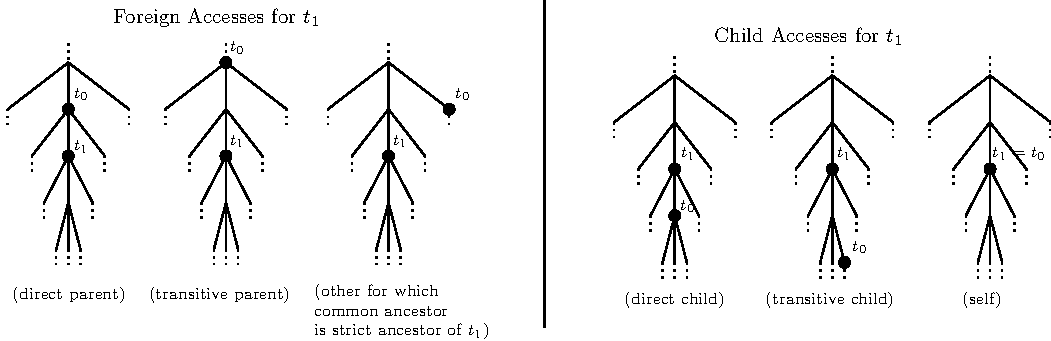
\includegraphics[width=\textwidth]{../figs/accesses-kinds.pdf}
    \caption{Accesses are classified in two categories depending on their relative position
    to the current tag. An access done through a (transitive and inclusive) child tag is a child access.
    An access done through a non-child tag (strict ancestor or non-comparable) is a foreign access.}
    \label{fig:kinds-of-accesses}
\end{figure}


\subsection{Pointer permissions}

\subsubsection{Available permission combinations}

Analysis of the different kinds of pointers leads us to choosing to give pointers
a permission among the following:
\begin{lstlisting}[language=rust]
enum ReadWritePerms {
    Reserved, // Represents a two-phase borrow during its reservation phase
    Active, // Represents an activated (written to) mutable reference
    Frozen, // Represents a shared (immutable) reference
    Disabled, // Represents a dead reference
}
\end{lstlisting}

We choose to introduce \tperm{Reserved} permissions as a way for Tree Borrows to
natively handle two-phase borrows. \tperm{Reserved} does not directly allow write
accesses through this pointer, but it keeps a right to obtain such
write permissions later in the execution.

\subsubsection{two-phase for all borrows}

As we have explained, \tperm{Reserved} represents mutable references with
a two-phase borrow not yet activated.

Rather than limiting this behavior to two-phase borrows only, we choose in Tree
Borrows to make all mutable borrows behave in a uniform way: all mutable references
will wait until their first write access to claim their write permission (become \tperm{Active}),
and will allow shared read-only access in the meantime. If not for this, a lot
of code currently being written would not be accepted, such as some code that
follows the following pattern
\begin{lstlisting}[language=rust]
                               // More generally:
let ptr = vec.as_mut_ptr();  // - some mutable reborrow
if vec.len() > 0 {             // - use base pointer immutably
   do_stuff(ptr)               // - then use the reborrow
}
\end{lstlisting}

A concrete example currently in use in the standard library test suite:
\begin{lstlisting}[language=rust]
let mut x = 2;
let xref = &mut x;
let xraw = &mut *xref as *mut _; // create a mutable reborrow
let xshr = &*xref;
assert_eq!(*xshr, 2); // read-only usage of the base pointer
unsafe {
    *xraw = 4; // usage of the mutable reborrow
}
assert_eq!(x, 4);
\end{lstlisting}

Extending the behavior of two-phase borrows to all mutable borrows also serves
towards our goal of allowing all reorderings of read-only operations: it lets
us exchange reads through mutable (but not used mutably) references with each
other and with reborrows of other mutable references.

\subsubsection{Initialization}

The initial permissions depend of the type of borrow.
Recall from Section \ref{sec:tree-structure} that raw pointers do not receive new permissions and instead
use the same tag and permissions as their parent pointer. This leaves mutable and
shared references for which we must determine an initial permission.

All references allow read accesses initially. This is required
because we perform a fake read access upon reborrowing a reference, and it asserts
that all references are dereferenceable (they are tagged \tcode{dereferenceable}
in LLVM).

In addition, mutable references are allowed to eventually write,
so we initalized them to be \tperm{Reserved}, while shared references are
initialized as \tperm{Frozen}.

\subsection{Updates}
\label{sec:transitions}

We now describe how permissions are updated after an access is performed.
The update process is roughly as follows.

In reaction to an access at \tcode{t0}, traverse the tree. For each \tcode{t1} node of the
tree, if \tcode{t0} is a child of \tcode{t1} then the access is a child access at \tcode{t1}; otherwise
it is a foreign access at \tcode{t1}. Based on the type of access (both child/foreign
and read/write) and some local information, determine the new permissions for the
pointer.

\begin{figure}
    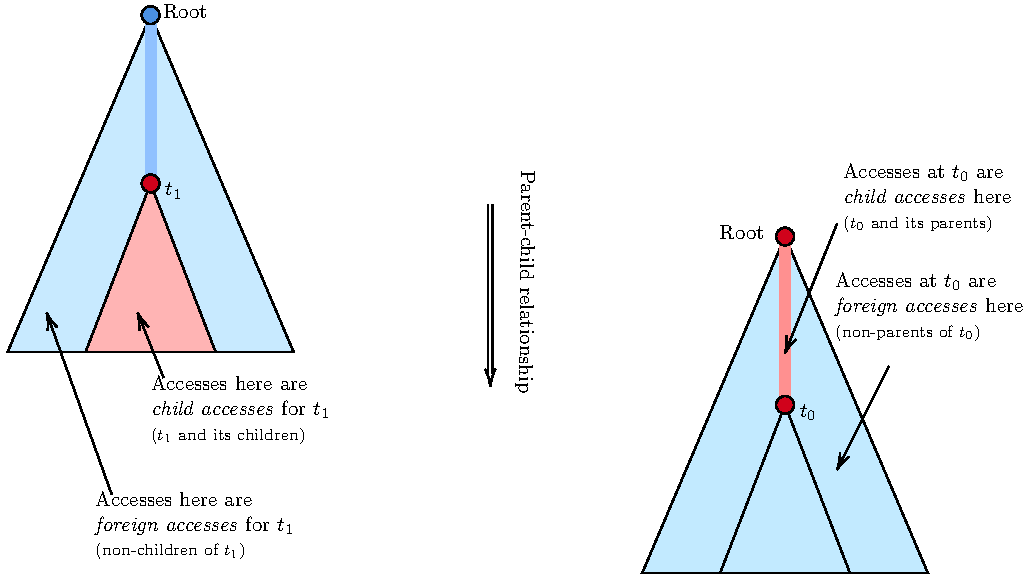
\includegraphics[width=\textwidth]{../figs/child-or-foreign.pdf}
    \caption{Two opposite points of view for the effects of an access.
    Left: how a given tag reacts to accesses at various positions.
    Right: how an access at a given position affects other tags.
    The foreign/child access naming follows the left convention which is easier
    for describing the update of permissions, but the right convention is closer
    to the actual implementation and better explains some optimizations.}
    \label{fig:access-pov}
\end{figure}

\subsubsection{Intuition on effects of accesses}
\label{sec:transitions-basic}

\paragraph*{Child accesses}

If \tperm{Active} is to represent mutable references, then it must allow child writes
as well as child reads. Our interpretation of \tperm{Reserved} as a mutable reference
that is not yet used mutably implies that it much be unaffected by child reads,
but turn into \tperm{Active} on the first child write.

\tperm{Frozen} representing a non-interior-mutable shared reference, it must allow
child reads. As child writes are forbidden on such references, we declare any
child write on a \tperm{Frozen} to be UB.

Any child access is obviously UB on a \tperm{Disabled} since dead references
do not allow accesses.

\paragraph*{Foreign accesses on Frozen}

Since shared references allow shared read access, \tperm{Frozen} must be unaffected
by foreign reads. As shared references on types without interior mutability
assume that no other reference accesses the same data mutably, a \tperm{Frozen} must
become \tperm{Disabled} upon a foreign write.

\paragraph*{Foreign accesses on Active}

Several mutable references cannot coexist with each other or with shared
references, so an \tperm{Active} must not remain \tperm{Active} upon a foreign access.

If another mutable reference is accessed, which corresponds to a foreign write,
then this \tperm{Active} must lose all permissions and become \tperm{Disabled}.

According to the Borrow Checker, an \tperm{Active} loses all permissions on a foreign read:
\begin{lstlisting}[language=rust]
// Example 3.A.1
fn main() {
    let base = &mut 42u64;
    let rmut = &mut *base;
    // base: Reserved
    // |-- rmut: Reserved
    *rmut += 1; // Child write for both base and rmut
    // base: Active
    // |--  rmut: Active
    let _val = *base; // Child read for base; foreign read for rmut
    // base: Active
    // |-- rmut: ???
    let _val = *rmut; // Compilation error
    // According to the Borrow Checker, rmut is no longer readable
}
\end{lstlisting}

However we want Tree Borrows to be suited for proving the validity of reordering
any two adjacent read accesses, which means in particular that reordering two
reads should not introduce new UB.

The following piece of code is accepted:
\begin{lstlisting}[language=rust]
// Example 3.A.2
fn main() {
    let base = &mut 42u64;
    let rmut = &mut *base;
    // base: Reserved
    // |-- rmut: Reserved
    *rmut += 1; // Child write for both base and rmut
    // base: Active
    // |--  rmut: Active
    let _val = *rmut; // Child read for both base and rmut
    // base: Active
    // |-- rmut: Active
    let _val = *base; // Child read for base; foreign read for rmut
    // base: Active
    // |-- rmut: ???
}
\end{lstlisting}
but swapping the two last reads from \textit{Example 3.A.2} would produce \textit{Example 3.A.1} above,
which would be UB if \tperm{Active} were to become \tperm{Disabled} on a foreign read.
We thus choose to make \tperm{Active} become \tperm{Frozen} instead, which means that in
both examples above \tperm{???} should be \tperm{Frozen} and UB occurs in neither.

\paragraph*{Foreign accesses on Reserved}
\label{sec:reserved}

\tperm{Reserved} is a more special case, and its behavior is guided by the following examples
(and more in Appendix \ref{app:reserved}):
\begin{lstlisting}[language=rust]
// Example 3.R.1: Foreign read (standard two-phase borrow example)
// This must not be UB
fn main() {
    let mut x = vec![];
    // x: Reserved
    x.push( // two-phase borrow starts here for x' implicitly reborrowed from x
        // x: Reserved
        // |-- x': Active
        x.len() // Foreign read for x'
        // After this, x' must still be writeable inside Vec::push
        // thus a foreign read must not affect Reserved tags.
    );
}

// Example 3.R.2: Foreign write
// This should be UB
fn main() {
    let mut x = 2;
    let mut xref = &mut x;
    // x: Reserved
    // |-- xref: Reserved
    *x = 3; // Child write for x; foreign write for xref
    // x: Active
    // |-- xref: ???
    *xref = 4; // If this is not UB then we are able to alternate writes
               // between two references that each claim exclusive access.
               // This is bad, so xref must no longer have write permissions.
               // The data has been mutated, so xref also can't claim shared
               // read-only access. Therefore foreign writes must make Reserved
               // turn into Disabled, which causes UB in this example as desired.
    *x = 3;
}

\end{lstlisting}

These suggest that a \tperm{Reserved} should tolerate foreign reads (stays \tperm{Reserved})
but not foreign writes (becomes \tperm{Disabled}). We have already established that
a \tperm{Reserved} allows child reads (stays \tperm{Reserved}) and must be changed
to \tperm{Active} before the first child write.


\subsubsection{Interpretation of transitions using an ordering}

From the conclusions of Section \ref{sec:transitions-basic} we can observe that all transitions follow the order
\tperm{Reserved < Active < Frozen < Disabled}, which corresponds to the permissions
during a ``normal'' lifetime of a mutable reference: it is \tperm{Reserved} upon creation
to accomodate for two-phase borrows, then eventually becomes \tperm{Active} on the first
child write. The next foreign read marks the end of its period of exclusive access
and it can now only be accessed immutably by becoming \tperm{Frozen}. Eventually its
lifetime ends altogether as a different branch claims exclusive access, it
becomes \tperm{Disabled} and will remain so forever.

A possible interpretation of the established transitions would be the following:
\begin{itemize}
    \item in reaction to a child access, the state will advance forward according to \tperm{<} until
        it has obtained the required read/write permissions for the access to be performed
        \begin{itemize}
            \item \tperm{Reserved}, \tperm{Active}, and \tperm{Frozen} already allow reading,
                so a child read does not affect them;
            \item \tperm{Active} also allows writing, so it is unaffected child Write;
            \item \tperm{Reserved} does not directly allow writing, but it can advance to \tperm{Active} to
                obtain the missing permission;
            \item \tperm{Frozen} for a write and \tperm{Disabled} for either a read or a write have no way of
                obtaining the required permissions, since all reachable states are also missing these
                permissions, this produces UB.
        \end{itemize}
    \item in reaction to a foreign access, the state will advance forward according to \tcode{<} until
        it has lost the incompatible read/write permissions
        \begin{itemize}
            \item \tperm{Disabled} having no permissions to lose, it has both many looping transitions and many incoming transitions;
            \item \tperm{Frozen} is the destination for an \tperm{Active} that needs to lose its write permission;
            \item \tperm{Frozen} and \tperm{Reserved} are compatible with a foreign read, hence the loops.
        \end{itemize}
\end{itemize}

In addition, notice that every state that has an incoming transition for any kind of
access also has a loop to itself for the same kind of access. For example a foreign read
access on \tperm{Active} leads to \tperm{Frozen}, which is stable under foreign reads. Similarly
a child write on Reserved leads to \tperm{Active} which is stable under child writes.
In other words, all transitions induced by accesses are idempotent.

This observation is an easy consequence of the ``advance until permissions are compatible''
interpretation of the transitions: once a state has been reached with compatible
permissions, applying the same access again will be a no-op because the state
is obviously already compatible. This idempotency of all accesses opens the door
for optimizations: if the consequences of a certain kind of access have already
been applied to some subtree of the borrow tree, said subtree can be skipped entirely
from the tree traversal if the next access is also of the same kind. This optimization
has been implemented and yields very noticeable improvements (x2 to x5 speedup).


\subsubsection{Protectors}
\label{sec:need-protect}

The compiler optimizations that Tree Borrows should justify include LLVM optimizations,
thus Tree Borrows must not allow violations of assumptions made by LLVM. Among these
assumptions is \tcode{noalias} which specifies to what extent a pointer passed as an
argument to a function aliases with other pointers. In Rust, mutable and shared
references in function arguments are both marked \tcode{noalias}.

\begin{figure}[h]
    \centering
    \begin{minipage}{0.8\textwidth}
        \tcode{noalias}

        This indicates that memory locations accessed via pointer values based on the argument
        are not also accessed, during the execution of the function, via pointer values not based on
        the argument. This guarantee only holds for memory locations that are modified,
        by any means, during the execution of the function.

        --- from the LLVM Language Reference Manual \cite{llvm_langref}
    \end{minipage}
\end{figure}

This can be reworded in language closer to Tree Borrows:

\begin{figure}[h]
    \centering
    \begin{minipage}{0.8\textwidth}
        An access via pointer values based on the argument is a \textbf{child access}.

        An access via pointer values \textbf{not} based on the argument is a \textbf{foreign access}.

        If a tag is marked noalias then during the execution of the function there must
        not be both child and foreign accesses relative to this tag if at least one of them is a write access.
    \end{minipage}
\end{figure}

This makes several pieces of code that would be allowed according to the model so
far be UB according to LLVM. Any code that is UB according to LLVM must also be
UB according to Rust. Examples of such code are shown in Appendix \ref{app:need-protect}.

To remedy this and properly detect this kind of UB, we introduce \textit{Protectors},
named after their Stacked Borrows equivalent.
Upon function entry, we add a Protector to every reference passed as argument, which
is now declared \textit{protected}. Protected pointers behave slightly differently from
unprotected pointers. Protectors are removed when the function returns.

This is implemented by maintaining a \tcode{HashSet} containing call ids of functions that have not yet
returned and their reference arguments, and querying this set on each transition
to know if this tag's permissions should follow the protected or unprotected
version of the transitions. In order to not declare too much UB, we also add
to each state a boolean field \tcode{accessed}, which is initially \tcode{false}
and becomes \tcode{true} on the first child access.

We apply the following rules to pointers that have an active protector
(when the protector is removed upon function exit, these rules no longer apply):

\begin{itemize}
    \item any transition \tperm{Frozen -> Disabled}, \tperm{Active -> Frozen},
        \tperm{Active -> Disabled}, \tperm{Reserved -> Disabled} on a permission of a protected
        pointer is UB;
    \item \tperm{Reserved} is affected by foreign reads and writes regardless of interior mutability,
        it always becomes \tperm{Frozen} after a foreign read and \tperm{Disabled} after a foreign write.
\end{itemize}

In terms of read/write permissions, this means that compared to the previous
model without protectors, additional UB occurs on any transition that causes
a loss of read or write permissions.
The transitions including protectors can be seen in the state automaton of Figure \ref{fig:state-machine}.

\begin{figure}
    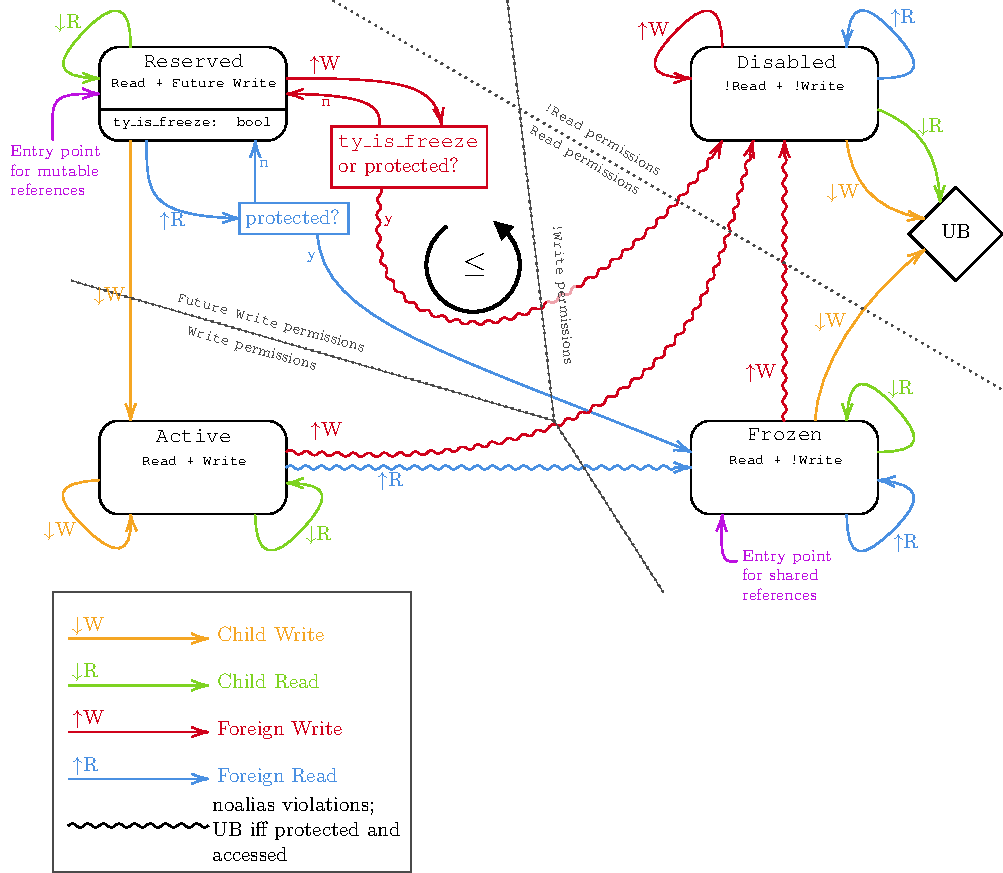
\includegraphics[width=\textwidth]{../figs/state-machine.pdf}
    \caption{State machine for the update of permissions including protectors}
    \label{fig:state-machine}
\end{figure}

\subsubsection{Accesses outside of initial range}

Tree Borrows is capable of handling pointers with unknown size as well as using
a pointer to access data outside of the range it was reborrowed for. One such case is
\begin{lstlisting}[language=rust]
fn access_after_offset() { unsafe {
    let data: [u64; 2] = [0, 1];
    let fst = &mut data[0] as *mut u64; // only reborrowed for [0]
    let snd = fst.add(1); // used on [1], which was not reborrowed
    ptr::swap(fst, snd);
} }
\end{lstlisting}
Here the reborrow for \tcode{fst} only covers \tcode{data[0]}, but \tcode{snd} is then derived from
\tcode{fst} and offset outside of its original range. As we still wish to check
that even for these accesses no aliasing assumptions are violated, we track
permissions even for locations outside of the range of the initial reborrow.

These permissions outside the range can be initialized lazily rather than as soon
as the reborrow occurs, because it is costly to immediately add permissions
on the entire allocation when they will most likely never be actually used by
a child access.

We do not perform a read access on reborrow for locations outside of the range.

\section{Tree Borrows implemented}

All behavior described here was implemented in Miri and is available since
\href{https://github.com/rust-lang/miri/pull/2785}{its recent merge} through
the \texttt{-Zmiri-tree-borrows} flag. Further testing and improvement
of diagnostics are scheduled.

\subsection{Testing the Rust Standard Library}
\label{sec:testing_stdlib}

We used the method described in
\href{https://github.com/rust-lang/miri-test-libstd}{\texttt{github:rust-lang/miri-test-libstd}}
to evaluate on the Standard Library that Tree Borrows does not declare ``too much UB'',
in other words that the code that is currently in use is not considered UB according
to Tree Borrows.

We found two tests that were rejected by Tree Borrows, both were instances of the
following pattern:
\begin{lstlisting}[language=rust]
let mut root = 6u8;        // Base pointer: Active
let mref = &mut root;      // Direct child: Reserved
let ptr = mref as *mut u8; // Uses the same tag as mref
// Write to ptr makes it Active
*ptr = 0;
// Parent read from the point of view of ptr makes it Frozen
assert_eq!(root, 0);
// Attempted write is rejected because Frozen forbids writes
*ptr = 0;
\end{lstlisting}

This pattern was previously accepted by Stacked Borrows, but has now been determined
to be arguably a violation of uniqueness that should not have been accepted in the
first place. It is also easy to patch: the fix (which simply consists of
replacing \tcode{\&mut root as *mut _} with \tcode{addr\_of\_mut!(root)}) was accepted
in \href{https://github.com/rust-lang/rust/pull/107954}{github:rust-lang/rust/pull/107954}.


Other widely used libraries such as \texttt{rand} and \texttt{tokio} already
satisfy the requirements of Tree Borrows, suggesting that most codebases will
need few to no changes if they are to enforce the Tree Borrows semantics.
Checking more thoroughly that this is actually the case is one of the ambitions of our future
work.

\subsection{Performance concerns and optimizations}
\label{sec:perf}

Tree Borrows is slower than Stacked Borrows.
The semantics require that on every access, every tag of the allocation have its
permissions updated on the corresponding range. On allocations with many reborrows
this can easily lead to a naive implementation of Tree Borrows being slower than
Stacked Borrows by an arbitrarily large multiplicative factor.


Fortunately Tree Borrows has access to easy optimizations that allow it to have
an execution time in the same order of magnitude as that of Stacked Borrows on
realistic code samples. We observe in Figure \ref{fig:perf} that in practice the slowdown from Stacked Borrows
to Tree Borrows is mostly less than x2 on benchmarks that are specifically designed
to stress the borrow tracker, and about x1.3 on general tests that don't particularly attempt to
push the borrow tracker to its limits.

Note further that the benchmarks that follow compare a very optimized implementation
of Stacked Borrows with a Tree Borrows implementation that was only optimized up to
the point that it would not waste too much time. Fine-tuning the garbage collector
of unused tags and implementing a cache are likely to improve the performance of
Tree Borrows as they have already done for Stacked Borrows.


\begin{figure}
    \centering
    \begin{tabular}{|l|l|c|c|c|c|}
        \hline
        Project & Test & Runs & SB & TB & Factor \\
        \hline
        \multirow{2}{9em}{Miri}
            & \texttt{slice-get-unchecked} & 5 & 0.56s & 4.15s & {\color{Red}x7.41} \\
            & \texttt{mse} & 5 & 0.67s & 1.42s & {\color{Red}x2.12} \\
            & \texttt{serde1} & 5 & 1.53s & 2.60s & {\color{YellowOrange}x1.70} \\
            & \texttt{serde2} & 5 & 3.19s & 5.16s & {\color{YellowOrange}x1.62} \\
            & \texttt{unicode} & 5 & 1.27s & 1.99s & {\color{YellowOrange}x1.57} \\
            & \texttt{backtraces} & 5 & 4.01s & 5.81s & {\color{YellowOrange}x1.45} \\
        \hline
        \multirow{3}{9em}{Stdlib}
            & \texttt{core} & 1 & 4m31s & 9m15s & {\color{Red}x2.05} \\
            & \texttt{alloc} & 1 & 4m45s & 5m54s & {\color{LimeGreen}x1.24} \\
            & \texttt{std/time} & 1 & 15.1s & 17.5s & {\color{LimeGreen}x1.16} \\
        \hline
        \multirow{1}{9em}{Regex}
            & \texttt{lib} & 1 & 13.3s & 20.6s & {\color{YellowOrange}x1.54} \\
        \multirow{1}{9em}{Hashbrown}
            & \texttt{lib} & 1 & 31.5s & 38.3s & {\color{LimeGreen}x1.21} \\
        \multirow{1}{9em}{Tokio}
            & \texttt{lib} & 1 & 40.7s & 45.3s & {\color{LimeGreen}x1.11} \\
        \multirow{1}{9em}{Rand}
            & \texttt{lib} & 1 & 1m24s & 1m31s & {\color{LimeGreen}x1.08} \\
        \multirow{1}{9em}{Memchr}
            & \texttt{lib} & 1 & 2.1s & 2.2s & {\color{LimeGreen}x1.05} \\
        \multirow{1}{9em}{Slotmap}
            & \texttt{lib} & 1 & {\color{Red}Error} & 18m15s & {\color{LimeGreen}x?} \\

        \hline
    \end{tabular}
    \caption{
        Benchmarks comparing the execution time of various widely used test suites
        for Stacked Borrows (SB) or Tree Borrows (TB). The increase in computation time
        is shown to be rarely a lot more than a factor \(1.5\).
        Some of these projects use Stacked Borrows as part of their continuous integration
        pipeline, so switching to Tree Borrows is shown to be reasonable in terms of
        additional computational requirement.
        The Appendix \ref{app:perf} lists the commands and sources
        that were used for each of these benchmarks.
    }
    \label{fig:perf}
\end{figure}



\section{Future work}

\subsection{Evaluating Tree Borrows on more real-world code}

Merely evaluating Tree Borrows on the examples shown in Section \ref{sec:testing_stdlib}
is not sufficient for a complete picture of how Tree Borrows fits in the Rust
ecosystem. With the help of \href{https://github.com/rust-lang/crater}{\texttt{crater}}
we plan to run tests on a much more significant portion of the existing Rust code.

\subsection{Proving optimizations}

We show a sketch of how to use Tree Borrows to prove some reordering-based optimization.
Part of our future work will be an attempt to formalize and generalize the proof that follows
as well as others.
\begin{lstlisting}[language=rust]
fn example2_unopt(x: &u64) -> u64 {
    let val = *x;
    g(); // arbitrary (possibly unsafe) unknown code modeled by a function call
    val
}

fn example2_opt(x: &u64) -> u64 {
    g();
    *x // This optimization is a read/call reordering + value propagation
}
\end{lstlisting}

For the above reordering to be valid, the following needs to hold.
For any definition of \tcode{g}, for any context \(C\), if \(C[\texttt{example2\_unopt}]\)
does not exhibit UB then \(C[\texttt{example2\_opt}]\) also does not exhibit UB.
We call \(C[\texttt{example2\_unopt}]\) the source, and \(C[\texttt{example2\_opt}]\)
the target.

Proof sketch: it is sufficient to prove that if \tcode{example2\_unopt} and \tcode{example2\_opt}
are executed with the same memory state and initial borrow tree
for which \tcode{example2\_unopt} does not trigger UB then
\begin{itemize}
    \item \tcode{example2\_opt} does not trigger UB, and
    \item they both modify the memory in the same way, and
    \item they return the same value, and
    \item they result in the same final borrow tree.
\end{itemize}

Indeed if neither triggers UB immediately and they result in the same memory
state and borrow tree then the two versions of the function will be indistinguishable
without UB in the source.

We mark the following notable points of the code:
\begin{lstlisting}[language=rust]
fn example2_unopt(x: &u64) -> u64 {
    // s0
    let val = *x;
    // s1
    g();
    // s2
    val
    // s3
}

fn example2_opt(x: &u64) -> u64 {
    // t0
    g();
    // t1
    *x
    // t3
}
\end{lstlisting}
and denote \(T(x)\) and \(M(x)\) the tree and memory at the execution point \(x\).

Let \(l\) the location that \tcode{x} points to: \(M(s_0)[l]\) is the value
of \tcode{*x} at \(s_0\).

We first show that \tcode{g} must not perform a write to \(l\). We have created
a fresh tag \(p_x\) for \tcode{x} and no child tag of \(p_x\) has been passed
to \tcode{g}, thus any access that occurs during \tcode{g} is a foreign access
for \(p_x\). Since \(p_x\) is protected, any foreign write would be UB, thus
\tcode{g} can be assumed not to perform any write access to \(l\).
Therefore the value at \(l\) in unchanged during the execution of \tcode{g} in
the source. This proves that both functions return the same value.

Assuming \(M(s_0) = M(t_0)\) since the two functions are to be executed in the
same context, and since no write occurs at all between \(s_0\) and \(s_1\)
we thus obtain \(M(s_1) = M(t_0)\). In the source and the target the whole memory
is identical when \tcode{g} is called, thus \tcode{g} executes in the same way
in both. Since no memory modification occurs between \(s_2\) and \(s_3\) or between
\(t_1\) and \(t_3\), we obtain that \(M(s_3) = M(t_3)\).

What remains is to show that the source and target result in the same
borrow tree and that the target does not have UB. Since \(T(t_0)\) refines
\(T(s_1)\), no UB occurs in the target during the execution of \tcode{g}.
We then examine what happens to all borrows for the location:
\begin{itemize}
    \item \(p_x\) in the source is subjected to a child read then zero or more
        child reads during \tcode{g}. It does not matter the order, the final
        permission of \(p_x\) will be the same in the target, i.e. \tperm{Frozen};
    \item there are no children of \(p_x\);
    \item non-children of \(p_x\) that already existed before the execution
        of the function are subjected in the target to the operations in \tcode{g}
        then a read of \(t_x\) instead of the opposite in the source. We easily
        check that in the state machine all transitions induced by read accesses
        (both child and foreign) commute with each other and thus the final
        permissions are the same in the source and in the target.
    \item non-children of \(p_x\) that were created during the execution of \tcode{g}
        are not protected when \tcode{*x} is read in the target and they are not
        \tperm{Active} because creating an \tperm{Active} requires a write.
        The read is thus a no-op.
\end{itemize}

We have thus shown that in the absence of UB in the source,
\(T(s_0) = T(t_0) \Longrightarrow T(s_3) = T(t_3)\) and
thus the source and target have the same behavior, and moving a read access
down across unknown code within a function is a valid optimization.

\subsection{Formalization}

Using the Simuliris framework \cite{simuliris} (Simuliris is derived from Iris which is derived from Coq)
we hope to be able to formally prove the above optimization and others.
This requires first formalizing Tree Borrows, and one difficulty is expected to be
the handling of parallelism: since Tree Borrows requires but does not directly implement
detection of race conditions (race conditions are UB, so the optimizations must
not introduce race conditions), the formalization will need to either consider
only a sequential language or include a race condition detection algorithm from prior work.


% ------------------------------------------------------------------------------

\newpage

\bibliography{literature}


\appendix

\newpage
\section{Benchmarks for Section \ref{sec:perf}}
\label{app:perf}

The benchmarks from Figure \ref{fig:perf} were executed with the following commands.
By default Stacked Borrows is used, and Tree Borrows is selected by appending
\texttt{-Zmiri-tree-borrows} to the list of \texttt{MIRIFLAGS}.

\begin{itemize}
    \item Miri\\
        These benchmarks are designed specifically to exhibit pathological behaviors of
        Stacked Borrows. It happens that many of these are also pathological cases for Tree Borrows,
        in particular very narrow trees (stack-like, obtained by chaining many reborrows)
        and very wide trees (obtained by reborrowing many times from the same pointer).
        It is within expectations that Tree Borrows would perform worse in comparison
        to Stacked Borrows on these tests than on other tests.
        \begin{description}
            \item[Source] \href{https://github.com/rust-lang/miri}{\texttt{github:rust-lang/miri}}
            \item[Command] \texttt{MIRIFLAGS="" ./miri bench}
        \end{description}
    \item Miri-test-libstd\\
        These tests constitute the OS-independent test suites of the Rust standard library. They
        are already used to detect regressions in either Miri or Rustc, but this check currently
        uses Stacked Borrows and not Tree Borrows.
        \begin{description}
            \item[Source] \href{https://github.com/rust-lang/miri-test-libstd}{\texttt{github:rust-lang/miri-test-libstd}}
            \item[Command] \texttt{MIRIFLAGS="" ./run-test.sh core --lib --tests}
            \item[Command] \texttt{MIRIFLAGS="" ./run-test.sh alloc --lib --tests}
            \item[Command] \texttt{MIRIFLAGS="-Zmiri-disable-isolation"}\\
                \texttt{./run-test.sh std --lib --tests -- time::}
        \end{description}
    \item Tokio\\
        This crate is a framework for writing asynchronous code. Since it uses \tcode{unsafe} and
        parallelism in nontrivial ways, detecting UB is important.
        \begin{description}
            \item[Source] \href{https://github.com/tokio-rs/tokio}{\texttt{github:tokio-rs/tokio}}
            \item[Command] \texttt{MIRIFLAGS="-Zmiri-disable-isolation -Zmiri-tag-raw-pointers"} \\
                \texttt{cargo +nightly miri test --features full --lib}
        \end{description}
    \item Rand\\
        This crate is the most widely used crate for random number generation.
        Rand is historically relevant to one of the main
        issues \cite{issue_raw_range_strict}
        of Stacked Borrows' handling of out-of-range raw pointers.
        \begin{description}
            \item[Source] \href{https://github.com/rust-random/rand}{\texttt{github:rust-random/rand}}
            \item[Command] \texttt{MIRIFLAGS="" cargo +nightly miri test --lib}
        \end{description}
    \item Hashbrown\\
        This crate implements a high-performance hash map, which naturally involves aliasing and \tcode{unsafe}.
        \begin{description}
            \item[Source] \href{https://github.com/rust-lang/hashbrown}{\texttt{github:rust-lang/hashbrown}}
            \item[Command] \texttt{MIRIFLAGS="" cargo +nightly miri test --lib}
        \end{description}
    \item Regex\\
        As the name suggests this is a crate for parsing, compiling, and executing regular expressions.
        The test \texttt{encode\_decode} is ignored because it takes too long for Miri to execute.
        \begin{description}
            \item[Source] \href{https://github.com/rust-lang/regex}{\texttt{github:rust-lang/regex}}
            \item[Command] \texttt{MIRIFLAGS="" cargo +nightly miri test --lib -- --skip encode\_decode}
        \end{description}
    \item Memchr\\
        High-performance implementation of standard string search primitives.
        Historically had a conflict with Stacked Borrows as stated in
        \href{https://github.com/BurntSushi/memchr/issues/58}{Issue \#58}
        \begin{description}
            \item[Source] \href{https://github.com/BurntSushi/memchr}{github:BurntSushi/memchr}
            \item[Command] \texttt{MIRIFLAGS="" cargo +nightly miri test}
        \end{description}
    \item Slotmap\\
        General purpose maps. Currently has an open \href{https://github.com/orlp/slotmap/issues/92}{Issue \#92}
        showing that some tests contain UB according to Stacked Borrows but not Tree Borrows.
        \begin{description}
            \item[Source] \href{https://github.com/orlp/slotmap}{github:orlp/slotmap}
            \item[Command] \texttt{MIRIFLAGS="" cargo +nightly miri test --lib}
        \end{description}
\end{itemize}

\newpage
\section{Requirements of protectors}
\label{app:need-protect}

To show why protectors are needed and why they require some alternative
transitions, we show here examples of programs that are UB according to LLVM,
but would not be UB according to Tree Borrows \textbf{if protected pointers behaved identically to unprotected pointers}.
This is a continuation of the example shown in Section \ref{sec:need-protect}.

\subsection{Increased requirements of \tperm{Reserved}}

The following program justifies that after a foreign read has occured, \tperm{Reserved} must no longer allow
foreign reads. Indeed if \tperm{Reserved} is unaffected by foreign reads then it allows a foreign read
followed by a child write. We model this by making \tperm{Reserved} become \tperm{Frozen} on a foreign read,
which means that the next attempted child write would correctly be UB.

For the same reason \tperm{Reserved} must not stay \tperm{Reserved} after a foreign write even
if it has interior mutability: we declare that under a foreign write, \tperm{Reserved} becomes
\tperm{Disabled} regardless of interior mutability which means that the next attempted child read or write would be UB.

\begin{lstlisting}[language=rust]
fn main() {
    let data = &mut 42u64;
    let y = data as *const u64;
    let x = &mut *data;
    foreign_read_before_write(x, y);
    fn foreign_read_before_write(x: &mut u64, y: *const u64) {
        // x: Reserved [noalias]
        let _ = unsafe { *y }; // Foreign read for x
        // x: Reserved [noalias]
        *x += 1; // Child write for x
        // /!\ Combined with the previous foreign read this is a noalias violation
        // x: Active [noalias]
        // -- UB must occur before this point --
        // (Without protectors no UB occurs)
    }
}
\end{lstlisting}


\subsection{Loss of read permissions}

A \tperm{Frozen} pointer becoming \tperm{Disabled} is a symptom that a foreign write occured after
a child read. Indeed a foreign write is only possible cause of the transition in question.
If the location was also accessed through any child access, then these two accesses violate
\tcode{noalias}, thus a transition \tperm{Frozen -> Disabled} should be UB on any accessed location.
The same remark applies to a \tperm{Reserved} or \tperm{Active} becoming \tperm{Disabled}.

\begin{lstlisting}[language=rust]
fn main() {
    let data = &mut 42u64;
    let y = data as *mut u64;
    let x = &*data;
    read_before_foreign_write(x, y);
    fn read_before_foreign_write(x: &u64, y: *mut u64) {
        // x: Frozen [noalias]
        let _ = *x; // Child read for x
        // x: Frozen [noalias]
        unsafe { *y += 1; } // Foreign write for x
        // /!\ Combined with the previous child read this is a noalias violation
        // x: Disabled [noalias]
        // -- UB must occur before this point --
        // (Without protectors no UB occurs)
    }
}
\end{lstlisting}


\subsection{Loss of write permissions}

An \tperm{Active} pointer becoming \tperm{Frozen} indicates the presence of a child write
(requirement for the existence of an \tperm{Active}) and a foreign write (only possible cause
of the transition). These two accesses violate \tcode{noalias}, thus a transition \tperm{Active -> Frozen}
should be UB.

\begin{lstlisting}[language=rust]
fn main() {
    let data = &mut 42u64;
    let y = data as *const u64;
    let x = &mut *data;
    write_before_foreign_read(x, y);
    fn write_before_foreign_read(x: &mut u64, y: *const u64) {
        // x: Reserved [noalias]
        *x += 1; // Child write for x
        // x: Active [noalias]
        let _ = unsafe { *y }; // Foreign read for x
        // /!\ Combined with the previous child write this is a noalias violation
        // x: Frozen [noalias]
        // -- UB must occur before this point --
        // (Without protectors no UB occurs)
    }
}
\end{lstlisting}

\newpage
\section{Behavior of \tperm{Reserved}}
\label{app:reserved}

In addition to the examples shown in Paragraph \ref{sec:reserved}, about
\tperm{Reserved}, some details of the behavior are guided by the observations
that follow.

This pattern is used frequently in the standard library test suite,
it would preferably not be UB.
It consists of a read access through a raw pointer between the creation
and access of a mutable reference, and it illustrates why Tree Borrows
uses the \tperm{Reserved} permission for all mutable references and not
just for two-phase borrows.
\begin{lstlisting}[language=rust]
// Example: Foreign read outside two-phase borrow
// This should not be UB.
fn main() {
    let mut x = 2;
    let xref = &mut x;
    let xraw = &mut *xref as *mut _;
    let xshr = &*xref;
    // x: Reserved
    // |-- xref: Reserved
    //     |-- xraw: Reserved
    //     |-- xshr: Frozen
    assert_eq!(*xshr, 2); // This is a foreign read for xref and xraw
    unsafe { *xraw = 4; } // This is a child write for xref and xraw
                          // meaning it must still be writeable at this point,
                          // therefore the above foreign read must not have turned
                          // them Frozen.
    assert_eq!(x, 4);
}
\end{lstlisting}


This second pattern shows that mutable references that involve interior mutability
must be exempt from the rule that a \tperm{Reserved} is disabled upon a foreign
write. This is safe code, it must absolutely not be UB.
\begin{lstlisting}[language=rust]
// Example: Foreign write with interior mutability
// This must not be UB
fn main() {
    use std::cell::Cell;
    trait Thing: Sized {
        fn do_the_thing(&mut self, _s: ());
    }

    let mut x = Cell::new(1);
    // x: Reserved
    x.do_the_thing({
        // A two-phase borrow starts here for x' implicitly reborrowed from x
        // x: Reserved
        // |-- x': Reserved
        x.set(3) // This is a foreign write for x'
        // x: Active
        // |-- x': ???
    })
    impl<T> Thing for Cell<T> {
        fn do_the_thing(&mut self, _s: ()) {
            // Function call starts, x' is implicitly reborrowed into x''
            // x: Active
            // |-- x': ???
            //     |-- x'': Reserved
            self.set(5): // x' must be readable and writeable
                         // This is a child write for x', which means
                         // that x' is now Active and was not previously Disabled
                         // or Frozen. Therefore x' was previously still Reserved,
                         // even though it was subjected to a foreign write.
        }
    }
}
\end{lstlisting}



\newpage
\section{Summary of the model}

Below is a summary of the points established in \ref{sec:tree_additions} and \ref{sec:transitions}
as a full description of Tree Borrows.

\paragraph*{When creating a new pointer \tcode{z} from an existing \tcode{y}}
\begin{itemize}
    \item if \tcode{z} is a \tcode{Unpin} mutable reference
        \begin{itemize}
            \item perform the effects of a read access through \tcode{y} on the reborrowed range
            \item add a new child of \tcode{y} in the tree
            \item give it the permissions \tperm{Reserved}
                (immediately on the reborrowed range, lazily on the rest of the allocation)
            \item keep track of whether it has interior mutability or not
        \end{itemize}
    \item if \tcode{z} is a non-interior-mutable shared reference
        \begin{itemize}
            \item perform the effects of a read access through \tcode{y} on the reborrowed range
            \item add a new child of \tcode{y} in the tree
            \item give it the permissions \tperm{Frozen}
                (immediately on the reborrowed range, lazily on the rest of the allocation)
        \end{itemize}
    \item otherwise give \tcode{z} the same tag as \tcode{y}, they are indistinguishable from now on
\end{itemize}

\paragraph*{When reading through a pointer \tcode{y}}
\begin{itemize}
    \item for all ancestors \tcode{x} of \tcode{y} (including \tcode{y}), this is a child read
        \begin{itemize}
            \item assert that \tcode{x} has read permissions (i.e. is \tperm{Frozen} or \tperm{Reserved} or \tperm{Active})
            \item otherwise (if \tcode{x} is \tperm{Disabled}) this is UB
        \end{itemize}
    \item for all non-ancestors \tcode{z} of \tcode{y} (excluding \tcode{y}), this is a foreign read
        \begin{itemize}
            \item turn \tperm{Active} into \tperm{Frozen}; this is UB if \tcode{z} is protected
            \item if \tcode{z} is protected, turn \tperm{Reserved} into \tperm{Frozen}
        \end{itemize}
\end{itemize}

\paragraph*{When writing through a pointer \tcode{y}}
\begin{itemize}
    \item for all ancestors \tcode{x} of \tcode{y} (including \tcode{y}), this is a child write
        \begin{itemize}
            \item turn \tperm{Reserved} into \tperm{Active}
            \item it is UB to encounter either \tperm{Disabled} or \tperm{Frozen}
        \end{itemize}
    \item for all non-ancestors \tcode{z} of \tcode{y} (excluding \tcode{y}), this is a foreign write
        \begin{itemize}
            \item if \tcode{z} is protected this is always UB; otherwise
            \item if \tcode{z} is \tperm{Reserved} and has interior mutability it is unchanged; otherwise
            \item turn all of \tperm{Reserved}, \tperm{Active}, and \tperm{Frozen} into \tperm{Disabled}.
        \end{itemize}
\end{itemize}

\end{document}
